\section{Nicole Oresme: The Birth of Mathematical Relationships (1350s)}

\textbf{But what if motion wasn’t just a distortion of some divine perfection? What if it could be studied as a relationship between changing quantities?}

For over a thousand years, Neoplatonism and Aristotelian physics dominated how people thought about the universe. Motion was seen as either an imperfection of reality or something tied to an object’s nature, rather than something that could be mathematically analyzed.

Then came \textbf{Nicole Oresme (1350s)}, a medieval scholar who made a radical leap.

\subsection{A New Way to Think About Motion: One Quantity Depending on Another}

Oresme proposed something that seems obvious today, but was groundbreaking at the time:

\begin{quote}
\textit{A quantity can change as another quantity changes.}
\end{quote}

This was a complete break from previous ways of thinking.

\begin{itemize}
    \item Plato and the Neoplatonists saw mathematics as \textbf{static truths}, existing beyond the physical world.
    \item Aristotle viewed motion as something dictated by an object’s \textbf{intrinsic nature}.
    \item Oresme saw motion as a \textbf{mathematical relationship}—a dynamic connection between two varying quantities.
\end{itemize}

For example, Oresme studied how speed changes over time and represented this variation graphically, centuries before Cartesian coordinates were invented.

\textbf{But how do you represent change mathematically?}

\subsection{Oresme’s Graphical Breakthrough: The First Step Toward Functions}

Oresme developed an \textbf{early form of graphing}, where one quantity was plotted against another.

\begin{center}
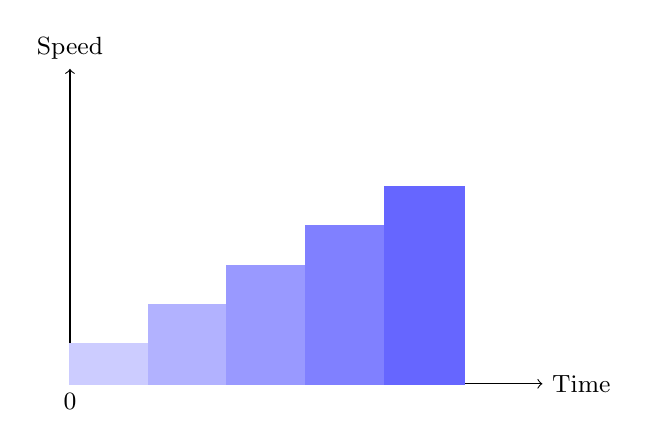
\begin{tikzpicture}
    % Axes
    \draw[->] (0,0) -- (6,0) node[right] {\small Time};
    \draw[->] (0,0) -- (0,4) node[above] {\small Speed};

    % Rectangles representing increasing speed over time
    \filldraw[blue!20, thick] (0,0) rectangle (1,0.5);
    \filldraw[blue!30, thick] (1,0) rectangle (2,1);
    \filldraw[blue!40, thick] (2,0) rectangle (3,1.5);
    \filldraw[blue!50, thick] (3,0) rectangle (4,2);
    \filldraw[blue!60, thick] (4,0) rectangle (5,2.5);

    % Labels
    \node[below] at (0,0) {\small 0};


\end{tikzpicture}
\end{center}



This was the first step toward the modern concept of a function—though he lacked the notation to express it algebraically.

